\subsection{Ikonok}

%_
\begin{frame}
  Ikonok:
  \begin{itemize}
    \item feldobják az oldal megjelenését
    \item lényegretörő, kifejező
  \end{itemize}
  \vfill
  Használat: \texttt{<i>} vagy \texttt{<span>} elemek + \texttt{class} attribútum
  \vfill
  CSS-sel formázhatóak: méret, szín, árnyék, szegély, stb.
  \vfill
  Több ikon könyvtár is elérhető.
\end{frame}

%_
\begin{frame}
  \hiv{\href{https://fontawesome.com}{Font Awesome}}
  \begin{itemize}
    \item 1588 ikon ingyen + 7842 fizetős
    \item Kit kódot kell igényelni a használathoz (az enyém pl. 5e6bd4a2fc)
    \item Egy \texttt{<script>} elemet kell beszúrni az oldalba a használathoz
    \item \texttt{class} attribútum értékei az ikonkészlet választáshoz:
    \begin{itemize}
      \item \texttt{fas} $\to$ Font Awesome Solid
      \item \texttt{fab} $\to$ Font Awesome Brand
      \item \texttt{Regular}, \texttt{Light}, \texttt{Duotone} a fizetős változatban
    \end{itemize}
    \item \texttt{class} attribútum értékei méretezéshez (enélkül a betűmérethez igazodik):
    \begin{itemize}
      \item \texttt{fa-xs}, \texttt{fa-sm}, \texttt{fa-lg}
      \item \texttt{fa-2x}, \texttt{fa-3x}, \dots, \texttt{fa-10x}
    \end{itemize}
  \end{itemize}
\end{frame}

%
\begin{frame}
  \begin{itemize}
    \item Léteznek azonos szélességű ikonok, pl. függőlegesen elrendezett menühöz (\texttt{fa-fw})
    \item Felsorolásjelekként állhatnak (pl. \texttt{fa-ul}, \texttt{fa-li}, \texttt{fa-check-square})
    \item Forgathatóak, tükrözhetőek (pl. \texttt{fa-rotate-90}, \texttt{fa-flip-vertical})
    \item Animálhatóak (\texttt{fa-spin}, \texttt{fa-pulse})
    \item Fizetős változat további szolgáltatásokkal: méretezés, pozicionálás, maszkolás, rétegek, \dots
    \item Egy lehetséges alternatíva: \hiv{\href{https://icons8.com/line-awesome}{Line Awesome}}
  \end{itemize}
\end{frame}

%_
\begin{frame}
  \begin{columns}[c]
    \column{0.76\textwidth}
      \begin{exampleblock}{\textattachfile{fontawesome.html}{fontawesome.html}}
        \scriptsize
        \lstinputlisting[style=HTML,linerange={7-8},numbers=left,firstnumber=7]{fontawesome.html}
        \lstinputlisting[style=HTML,linerange={12-23},numbers=left,firstnumber=12]{fontawesome.html}
      \end{exampleblock}
    \column{0.2\textwidth}
      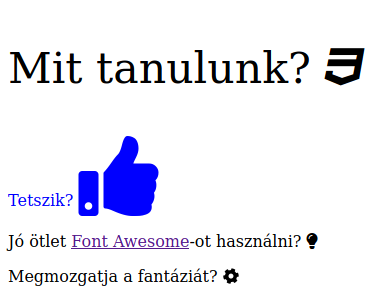
\includegraphics[width=\textwidth]{fontawesome.png}
  \end{columns}
\end{frame}

%_
\begin{frame}
  Google Material Icons
  \begin{itemize}
    \item Egységes, letisztult UI készítéséhez használható ikonkészlet, és UI tervezési elvek
    \item Kevesebb ikon, egyszerűbb szolgáltatások, ligatúrákat használ.
    \item \hiv{\href{https://material.io/resources/icons}{Ikonlista}}
    \item \hiv{\href{https://google.github.io/material-design-icons/}{Felhasználási útmutató}}
    \item Egy stíluslap betöltése után használható
    \item Az oldal szerkesztőjének kell stílusokat definiálni a méretezéshez (pl. \texttt{md-48}), színezéshez (pl. \texttt{md-dark}), stb.
  \end{itemize}
\end{frame}

%_
\begin{frame}
  \begin{columns}[c]
    \column{0.76\textwidth}
      \begin{exampleblock}{\textattachfile{material.html}{material.html}}
        \scriptsize
        \lstinputlisting[style=HTML,linerange={6-12},numbers=left,firstnumber=6]{material.html}
        \lstinputlisting[style=HTML,linerange={24-29},numbers=left,firstnumber=24]{material.html}
      \end{exampleblock}
    \column{0.2\textwidth}
      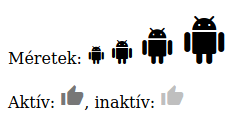
\includegraphics[width=\textwidth]{material.png}
  \end{columns}
\end{frame}
